\documentclass[12pt,a4paper]{article}

% ============================================================
% PACOTES
% ============================================================

\usepackage[utf8]{inputenc}
\usepackage[T1]{fontenc}
\usepackage[brazil]{babel}

\usepackage{geometry}
\usepackage{graphicx}
\usepackage{float}
\usepackage{booktabs}
\usepackage{array}
\usepackage{longtable}

\usepackage{amsmath}
\usepackage{amssymb}

\usepackage{xcolor}
\usepackage{listings}

\usepackage{enumitem}

\usepackage[
    hidelinks
]{hyperref}

\usepackage{setspace}

\geometry{
    top=2.5cm,
    bottom=2.5cm,
    left=3cm,
    right=2cm
}

\setlength{\parindent}{1.25cm}
\setlength{\parskip}{0.2cm}

\onehalfspacing


% ============================================================
% CONFIGURAÇÃO DE CÓDIGO
% ============================================================

\lstset{
    language=Python,
    basicstyle=\ttfamily\small,
    numbers=left,
    numberstyle=\tiny,
    stepnumber=1,
    numbersep=8pt,
    showstringspaces=false,
    breaklines=true,
    frame=single,
    tabsize=4,
    captionpos=b
}


% ============================================================
% FIGURAS COM PLACEHOLDER
% ============================================================
%
% \Figura{arquivo.png}{legenda}{rotulo}
%
% Enquanto o arquivo nao existir na pasta do relatorio, e desenhada uma
% caixa indicando qual imagem deve ser colocada ali. Basta salvar o PNG
% com o nome indicado dentro desta pasta e recompilar: a figura entra no
% lugar da caixa sozinha, sem precisar editar o .tex.

\newcommand{\Figura}[3]{%
    \begin{figure}[H]
        \centering
        \IfFileExists{#1}{%
            \includegraphics[width=0.95\textwidth]{#1}%
        }{%
            \fbox{%
                \parbox[c][5cm][c]{0.9\textwidth}{%
                    \centering
                    \textbf{[ INSERIR FIGURA ]}
                    \par\vspace{0.4cm}
                    \texttt{\detokenize{#1}}
                    \par\vspace{0.4cm}
                    \small #2
                }%
            }%
        }
        \caption{#2}
        \label{#3}
    \end{figure}
}


% ============================================================
% DOCUMENTO
% ============================================================

\begin{document}


% ============================================================
% CAPA
% ============================================================

\begin{titlepage}

    \noindent
    \begin{minipage}[t]{0.15\textwidth}
        \vspace{0pt}
        
\includegraphics[width=2.2cm]{logo_uerj.jpg}
    \end{minipage}
    \hfill
    \begin{minipage}[t]{0.82\textwidth}
        \vspace{0pt}
        \raggedright

        {\large \textbf{Universidade do Estado do Rio de Janeiro}}\\[0.15cm]

        Departamento de Engenharia de Sistemas e Computação\\[0.15cm]

        Arquitetura de Sistemas Operacionais -- Turma 1
    \end{minipage}

    \vfill

    \begin{center}

        {\Large
        \textbf{
        Trabalho 1 -- Implementando um Simulador de Escalonamento
        }
        }

        \vspace{2.5cm}

        {\large
        \textbf{Giulia Campos}\\
        \textbf{Petro Liporace}
        }

        \vspace{2cm}

        \begin{flushright}
            \begin{minipage}{0.55\textwidth}

                Trabalho apresentado à disciplina de
                Arquitetura de Sistemas Operacionais,
                ministrada pela Prof.\textsuperscript{a}
                Rafaela Brum.

            \end{minipage}
        \end{flushright}

    \end{center}

    \vfill

    \begin{center}
        Rio de Janeiro\\
        23 de agosto de 2026
    \end{center}

\end{titlepage}


% ============================================================
% SUMÁRIO
% ============================================================

\tableofcontents

\newpage


% ============================================================
% 1. INTRODUÇÃO
% ============================================================

\section{Introdução}

O escalonamento de processos é uma das atividades fundamentais
realizadas por um sistema operacional. Em um sistema multiprogramado,
diversos processos podem estar simultaneamente prontos para utilizar
o processador, sendo necessário definir qual deles terá acesso à CPU
em determinado instante.

O escalonador é responsável por realizar essa seleção de acordo com
um algoritmo previamente definido. Dependendo da estratégia adotada,
aspectos como prioridade, ordem de chegada, tempo de execução e
quantum disponível podem influenciar diretamente a ordem na qual os
processos são executados.

Além dos períodos de utilização da CPU, um processo pode realizar
operações de entrada e saída (E/S). Nesses casos, o processo deixa
temporariamente o processador e passa ao estado bloqueado enquanto
aguarda a conclusão da operação solicitada. Durante esse período,
outro processo pode utilizar a CPU.

Este trabalho apresenta o desenvolvimento de um simulador de
escalonamento de processos. A implementação foi construída
progressivamente, inicialmente considerando somente a utilização da
CPU e, posteriormente, adicionando preempção, diferentes níveis de
prioridade, operações de entrada e saída, geração automática de
processos e acompanhamento dos eventos ocorridos durante a
simulação.


% ============================================================
% 2. OBJETIVO
% ============================================================

\section{Objetivo}

O objetivo principal do trabalho foi desenvolver um simulador capaz
de representar, de forma didática, o funcionamento de algoritmos de
escalonamento utilizados por sistemas operacionais.

Entre os algoritmos considerados encontra-se obrigatoriamente o
escalonamento por filas multiníveis com retroalimentação, também
conhecido como \textit{Multilevel Feedback Queue} (MLFQ).

O simulador foi projetado de forma que seja possível acompanhar o
estado dos processos e das diferentes filas ao longo de cada unidade
de tempo da simulação.

Foram considerados como objetivos específicos:

\begin{itemize}

    \item representar os principais dados de um processo através de
    uma estrutura equivalente ao PCB;

    \item representar os estados assumidos por um processo durante
    sua execução;

    \item implementar filas de diferentes níveis de prioridade;

    \item implementar preempção baseada em quantum;

    \item implementar operações de entrada e saída;

    \item permitir a execução simultânea conceitual da CPU e dos
    dispositivos de E/S;

    \item gerar automaticamente processos com características
    aleatórias;

    \item registrar os eventos ocorridos durante a simulação;

    \item calcular o tempo de turnaround de cada processo.

\end{itemize}


% ============================================================
% 3. PREMISSAS
% ============================================================

\section{Premissas do Simulador}

Antes da implementação do simulador, foram estabelecidas algumas
premissas para definir de forma clara o comportamento esperado do
sistema.

Essas premissas também permitiram simplificar determinados aspectos
de um sistema operacional real, mantendo o foco nos conceitos de
escalonamento apresentados durante a disciplina.

\subsection{Unidade de tempo}

O simulador trabalha com unidades discretas de tempo.

A cada iteração do laço principal da simulação ocorre o avanço de uma
unidade de tempo global.

Durante uma mesma unidade de tempo podem ocorrer diferentes
atividades de forma conceitualmente paralela, como, por exemplo, um
processo utilizando a CPU enquanto outro processo realiza uma
operação de E/S.

\subsection{Tempo de CPU}

O tempo de CPU de um processo representa exclusivamente a quantidade
de unidades de tempo nas quais ele precisa efetivamente utilizar o
processador.

Portanto, o período em que um processo permanece bloqueado realizando
uma operação de entrada e saída não reduz seu tempo restante de CPU.

Por exemplo, um processo que necessita de 10 unidades de CPU e
realiza uma operação de E/S com duração de 5 unidades continua
necessitando de apenas 10 unidades efetivas de processamento.

Caso seja o único processo existente no sistema e realize uma única
E/S, seu tempo mínimo até a conclusão será:

\[
10 + 5 = 15 \text{ unidades de tempo}
\]

Entretanto, somente 10 dessas unidades correspondem à utilização da
CPU.

\subsection{Filas de prioridade}

Para o algoritmo de filas multiníveis com retroalimentação foram
utilizados três níveis principais:

\begin{table}[H]
    \centering
    \caption{Filas utilizadas pelo algoritmo MLFQ}
    \begin{tabular}{ccc}
        \toprule
        \textbf{Fila} &
        \textbf{Prioridade} &
        \textbf{Quantum} \\
        \midrule
        Alta  & 0 & 2 \\
        Média & 1 & 4 \\
        Baixa & 2 & 6 \\
        \bottomrule
    \end{tabular}
\end{table}

A prioridade de valor numérico menor representa maior prioridade.

Todos os novos processos são inicialmente inseridos na fila de alta
prioridade.

\subsection{Preempção}

Quando um processo utiliza integralmente o quantum disponível sem
terminar sua execução ou solicitar uma operação de E/S, ele sofre
preempção.

No algoritmo MLFQ adotado, o processo é então rebaixado para a fila
imediatamente inferior.

Dessa forma:

\[
Alta \rightarrow Media \rightarrow Baixa
\]

Um processo que já esteja na fila de baixa prioridade e utilize todo
o seu quantum retorna ao final da própria fila.

\subsection{Operações de entrada e saída}

Foram considerados três tipos de operação de entrada e saída:

\begin{table}[H]
    \centering
    \caption{Tipos de entrada e saída considerados}
    \begin{tabular}{cc}
        \toprule
        \textbf{Dispositivo} &
        \textbf{Duração adotada} \\
        \midrule
        Disco       & 3 u.t. \\
        Fita        & 7 u.t. \\
        Impressora  & 10 u.t. \\
        \bottomrule
    \end{tabular}
\end{table}

Os valores representam o período durante o qual o processo permanece
bloqueado aguardando a conclusão da respectiva operação.

O tempo de E/S é controlado separadamente do tempo de CPU.


% ============================================================
% 4. DESENVOLVIMENTO
% ============================================================

\section{Desenvolvimento do Simulador}

O desenvolvimento foi dividido em etapas. Essa abordagem permitiu
validar individualmente as principais partes do simulador antes da
adição de novas funcionalidades.

A estratégia adotada foi começar com um caso simplificado contendo
somente CPU e, posteriormente, aumentar progressivamente a
complexidade da simulação.


% ============================================================
% 4.1
% ============================================================

\subsection{Representação dos processos}

O primeiro passo foi definir quais informações deveriam ser
armazenadas para cada processo.

Para representar o PCB de forma simplificada, foram armazenados
dados como:

\begin{itemize}

    \item PID;

    \item PPID;

    \item instante de chegada;

    \item prioridade;

    \item estado atual;

    \item tempo total de CPU;

    \item tempo restante de CPU;

    \item quantidade de CPU já executada;

    \item quantum restante;

    \item fila de origem da execução atual;

    \item instante de término;

    \item eventos de entrada e saída.

\end{itemize}

A partir desses dados foi criada a classe \texttt{Processo}, que
centraliza o estado de cada processo durante toda a simulação.


% ============================================================
% 4.2
% ============================================================

\subsection{Estados dos processos}

Os estados foram representados através de uma enumeração.

Foram utilizados os seguintes estados:

\begin{description}

    \item[NOVO:] processo criado, porém ainda não admitido no sistema;

    \item[PRONTO:] processo disponível para execução e aguardando uma
    CPU;

    \item[EXECUTANDO:] processo atualmente utilizando a CPU;

    \item[BLOQUEADO:] processo aguardando a conclusão de uma operação
    de E/S;

    \item[TERMINADO:] processo que concluiu toda a sua execução.

\end{description}

A utilização de uma enumeração tornou explícitas as transições de
estado realizadas durante a simulação.


% ============================================================
% 4.3
% ============================================================

\subsection{Implementação inicial sem entrada e saída}

Antes de inserir operações de E/S, foi implementada uma primeira
versão contendo somente:

\begin{itemize}

    \item chegada dos processos;

    \item filas de prioridade;

    \item seleção do processo;

    \item execução da CPU;

    \item controle de quantum;

    \item preempção;

    \item rebaixamento entre filas;

    \item término dos processos.

\end{itemize}

Essa decisão permitiu verificar isoladamente se o algoritmo de
escalonamento estava correto.


% ============================================================
% 4.4
% ============================================================

\subsection{Admissão dos processos}

A cada unidade de tempo é verificado se algum processo possui
instante de chegada igual ao tempo atual da simulação.

Quando isso ocorre, o processo altera seu estado de \texttt{NOVO}
para \texttt{PRONTO} e é inserido na fila de alta prioridade.

% ============================================================
% 4.5
% ============================================================

\subsection{Seleção do processo}

Sempre que a CPU está livre, o escalonador procura um novo processo.

A busca respeita a seguinte ordem:

\[
FilaAlta > FilaMedia > FilaBaixa
\]

Assim, somente quando nenhuma tarefa está disponível na fila de alta
prioridade a fila média é consultada.

Da mesma forma, a fila baixa somente é utilizada quando as duas
anteriores estiverem vazias.

Dentro de cada fila, os processos seguem uma política FIFO.


% ============================================================
% 4.6
% ============================================================

\subsection{Controle do quantum}

Ao receber a CPU, o processo recebe o quantum correspondente à fila
na qual estava armazenado.

A cada unidade de CPU utilizada:

\begin{itemize}

    \item o tempo restante de CPU é decrementado;

    \item o tempo total já executado é incrementado;

    \item o quantum restante é decrementado.

\end{itemize}

De forma simplificada:

\begin{lstlisting}
processo.tempo_restante -= 1
processo.tempo_cpu_executado += 1
processo.tempo_quantum -= 1
\end{lstlisting}

Quando o quantum chega a zero e o processo ainda possui tempo de CPU
restante, ocorre uma preempção.


% ============================================================
% 4.7
% ============================================================

\subsection{Rebaixamento entre as filas}

No MLFQ utilizado, um processo que utiliza completamente a fatia de
tempo disponível é transferido para um nível inferior.

O comportamento implementado segue:

\begin{lstlisting}
se fila_atual == ALTA:
    mover para MEDIA

senao se fila_atual == MEDIA:
    mover para BAIXA

senao:
    retornar ao final da fila BAIXA
\end{lstlisting}

Esse mecanismo permite favorecer inicialmente processos com rajadas
curtas de CPU, enquanto processos que utilizam longos períodos de
processamento são gradativamente deslocados para filas de menor
prioridade.


% ============================================================
% 5. VALIDAÇÃO INICIAL
% ============================================================

\section{Validação do Algoritmo MLFQ}

Antes da inclusão das operações de entrada e saída, foi realizada uma
validação utilizando um exemplo resolvido em sala de aula.

Foram considerados os seguintes processos:

\begin{table}[H]
    \centering
    \caption{Processos utilizados para validação}
    \begin{tabular}{ccc}
        \toprule
        \textbf{Processo} &
        \textbf{Chegada} &
        \textbf{Tempo de CPU} \\
        \midrule
        P1 & 0 & 5 \\
        P2 & 0 & 4 \\
        P3 & 1 & 8 \\
        P4 & 4 & 6 \\
        \bottomrule
    \end{tabular}
\end{table}

Foram utilizadas filas com quantums iguais a 2, 4 e 6 unidades de
tempo.

A sequência produzida pelo simulador foi:

\begin{table}[H]
    \centering
    \caption{Sequência de execução obtida}
    \begin{tabular}{cc}
        \toprule
        \textbf{Intervalo} &
        \textbf{Processo} \\
        \midrule
        0--2   & P1 \\
        2--4   & P2 \\
        4--6   & P3 \\
        6--8   & P4 \\
        8--11  & P1 \\
        11--13 & P2 \\
        13--17 & P3 \\
        17--21 & P4 \\
        21--23 & P3 \\
        \bottomrule
    \end{tabular}
\end{table}

Os processos foram finalizados nos seguintes instantes:

\begin{table}[H]
    \centering
    \caption{Tempos de término obtidos}
    \begin{tabular}{cc}
        \toprule
        \textbf{Processo} &
        \textbf{Término} \\
        \midrule
        P1 & 11 \\
        P2 & 13 \\
        P3 & 23 \\
        P4 & 21 \\
        \bottomrule
    \end{tabular}
\end{table}

Os resultados foram iguais aos apresentados no exercício feito em
sala, validando a lógica básica de chegada, seleção, quantum,
preempção, rebaixamento e contagem do tempo global.

\begin{figure}[H]
    \centering
    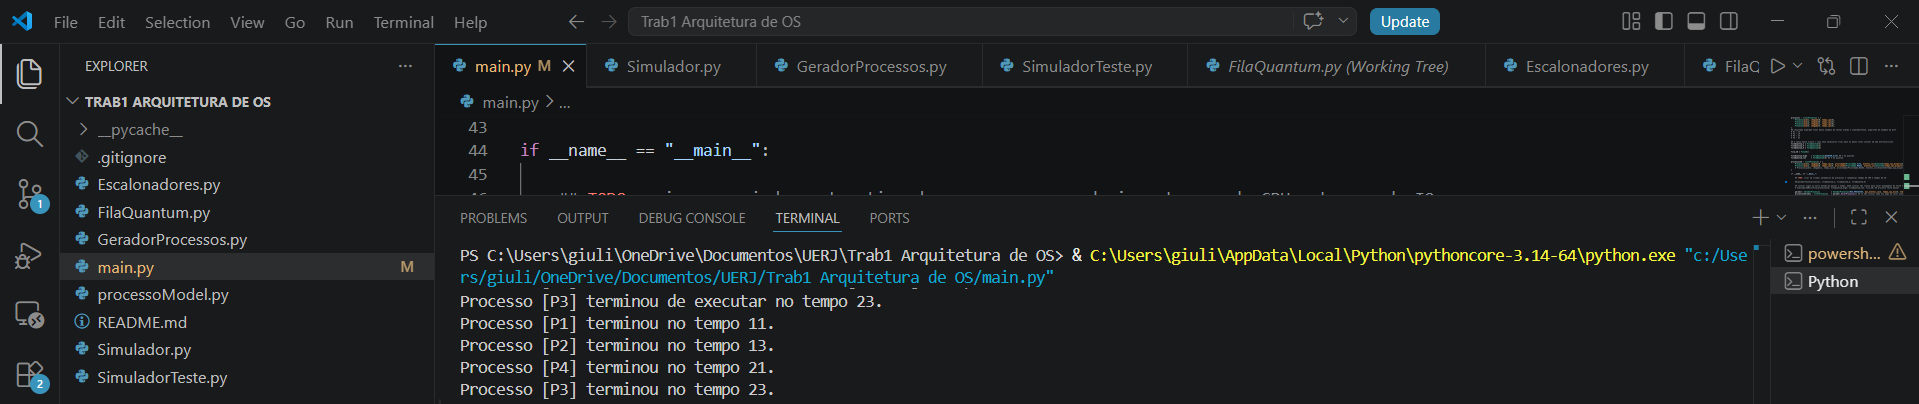
\includegraphics[width=0.8\textwidth]{processos.png}
    \caption{Resultado de teste do algoritmo MLFQ.}
    \label{fig:exemplo}
\end{figure}

% ============================================================
% 6. TURNAROUND
% ============================================================

\section{Cálculo do Turnaround}

O turnaround corresponde ao intervalo total entre a chegada de um
processo e sua conclusão.

Foi utilizada a expressão:

\[
T_{turnaround} =
T_{termino} -
T_{chegada}
\]

Para o teste inicial foram encontrados:

\[
P1 = 11 - 0 = 11
\]

\[
P2 = 13 - 0 = 13
\]

\[
P3 = 23 - 1 = 22
\]

\[
P4 = 21 - 4 = 17
\]

Portanto, o turnaround médio é:

\[
\frac{11+13+22+17}{4}
=
15,75
\]

Esse resultado também foi utilizado como um dos critérios de
validação da implementação.


% ============================================================
% 7. I/O
% ============================================================

\section{Adição das Operações de Entrada e Saída}

Após a validação do escalonamento sem E/S, a etapa seguinte consistiu
em incorporar operações de entrada e saída.

A principal decisão tomada nessa etapa foi separar completamente o
tempo de CPU do tempo utilizado pelos dispositivos de E/S.

Quando um processo solicita uma operação de E/S:

\begin{enumerate}

    \item ele deixa a CPU;

    \item seu estado passa para \texttt{BLOQUEADO};

    \item a operação é adicionada à respectiva fila de dispositivo;

    \item a CPU pode selecionar outro processo;

    \item o dispositivo de E/S é atualizado paralelamente ao
    processamento da CPU;

    \item quando a operação termina, o processo volta ao estado
    \texttt{PRONTO}.

\end{enumerate}


% ============================================================
% 7.1
% ============================================================

\subsection{Representação dos eventos de E/S}

Para permitir que um processo realize diversas operações de entrada e
saída ao longo de sua execução, foi criada a estrutura
\texttt{EventoIO}.

Cada evento contém:

\begin{itemize}

    \item o tipo de dispositivo;

    \item a quantidade de CPU já executada necessária para disparar a
    operação;

    \item a duração da operação.

\end{itemize}

Por exemplo, um processo com 20 unidades de CPU pode possuir:

\begin{table}[H]
    \centering
    \caption{Exemplo de eventos de E/S}
    \begin{tabular}{ccc}
        \toprule
        \textbf{CPU executada} &
        \textbf{Operação} &
        \textbf{Duração} \\
        \midrule
        5  & Disco      & 3 \\
        9  & Fita       & 7 \\
        14 & Impressora & 10 \\
        \bottomrule
    \end{tabular}
\end{table}

Nesse caso, o processo não solicita E/S em tempos globais
pré-determinados. O disparo depende da quantidade de CPU que o próprio
processo conseguiu efetivamente executar.

Isso é necessário porque um processo pode sofrer diversas
preempções antes de atingir o ponto de uma operação de E/S.


% ============================================================
% 7.2
% ============================================================

\subsection{Contadores independentes}

Foram mantidos contadores independentes para CPU e entrada e saída.

Enquanto o processo está executando:

\begin{lstlisting}
tempo_restante -= 1
tempo_cpu_executado += 1
tempo_quantum -= 1
\end{lstlisting}

Enquanto está bloqueado em E/S:

\begin{lstlisting}
tempo_io_restante -= 1
\end{lstlisting}

Assim, uma operação de E/S nunca reduz o tempo restante de CPU do
processo.


% ============================================================
% 7.3
% ============================================================

\subsection{Ordem de tratamento após uma unidade de CPU}

Após cada unidade de CPU, foi definida uma ordem para verificar os
eventos associados ao processo.

A prioridade adotada foi:

\begin{enumerate}

    \item verificar se o processo terminou;

    \item verificar se foi atingido um evento de E/S;

    \item verificar se o quantum foi completamente utilizado.

\end{enumerate}

Essa ordem evita, por exemplo, que um processo terminado seja
recolocado desnecessariamente em uma fila de prontos.


% ============================================================
% 8. GERAÇÃO AUTOMÁTICA
% ============================================================

\section{Geração Automática dos Processos}

Após a implementação da estrutura dos processos e dos eventos de
entrada e saída, foi criado um gerador automático de processos.

O objetivo dessa etapa foi evitar que a simulação dependesse
exclusivamente de processos definidos manualmente.

O gerador recebe parâmetros que estabelecem limites para a
simulação, como:

\begin{itemize}

    \item quantidade máxima de processos;

    \item quantidade máxima de eventos de E/S por processo;

    \item tempo mínimo de CPU;

    \item tempo máximo de CPU;

    \item menor instante possível de chegada;

    \item maior instante possível de chegada.

\end{itemize}


% ============================================================
% 8.1
% ============================================================

\subsection{Geração do tempo de serviço}

Para cada processo é sorteado um valor dentro do intervalo definido
para o tempo total de CPU.

Por exemplo:

\[
T_{CPU} \in [10,30]
\]

Dessa forma, diferentes processos podem apresentar diferentes
necessidades de processamento.


% ============================================================
% 8.2
% ============================================================

\subsection{Geração dos eventos de E/S}

A quantidade de operações de E/S também pode variar entre os
processos.

Se o número máximo permitido for três, um processo pode possuir:

\[
0,\;1,\;2\;\text{ou}\;3
\]

eventos.

Os pontos de disparo são selecionados dentro do intervalo:

\[
1 \leq T_{disparo} < T_{CPU}
\]

Isso garante que nenhuma operação seja programada depois do término
do processo.

Também são utilizados pontos distintos, impedindo que duas
solicitações diferentes de E/S sejam disparadas exatamente após a
mesma unidade de CPU.

Depois da geração, os eventos são ordenados de acordo com seu ponto de
disparo.


% ============================================================
% 8.3
% ============================================================

\subsection{Seleção aleatória do dispositivo}

Cada evento recebe aleatoriamente um dos tipos de E/S disponíveis:

\begin{itemize}

    \item disco;

    \item fita;

    \item impressora.

\end{itemize}

A partir do dispositivo escolhido é determinada a duração da operação.

\begin{figure}[H]
    \centering
    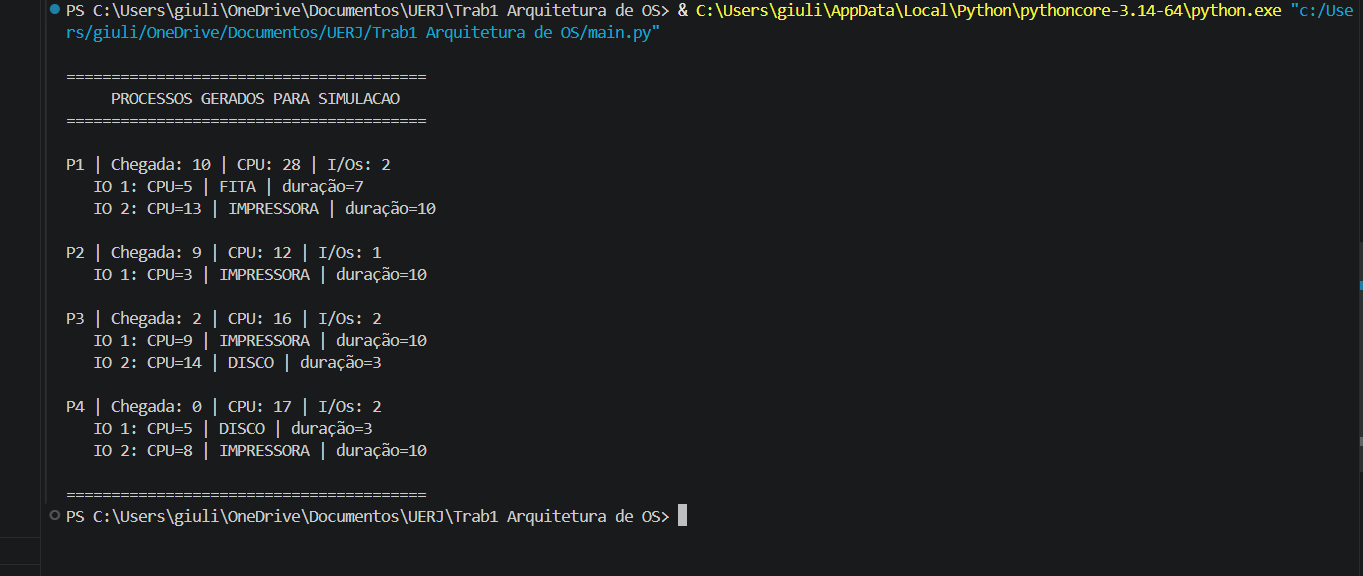
\includegraphics[width=\textwidth]{geracaoprocessoautomatico.png}
    \caption{Log dos processos aleatórios gerados}
    \label{fig:saida_simulador}
\end{figure}


% ============================================================
% 9. LOGS
% ============================================================

\section{Registro dos Eventos da Simulação}

Um dos objetivos do simulador é permitir que o funcionamento do
algoritmo seja acompanhado de forma didática.

Por esse motivo, foram adicionadas mensagens de log tanto no início
quanto durante a execução.


% ============================================================
% 9.1
% ============================================================

\subsection{Log dos processos criados}

Antes do início do escalonamento, são apresentadas informações de
todos os processos gerados.

Entre as informações exibidas estão:

\begin{itemize}

    \item PID;

    \item instante de chegada;

    \item tempo total de CPU;

    \item quantidade de eventos de E/S;

    \item instante de disparo de cada E/S em relação à CPU executada;

    \item dispositivo utilizado;

    \item duração da operação.

\end{itemize}

Um exemplo de saída é apresentado a seguir:

\begin{lstlisting}
P1 | Chegada: 2 | CPU: 20 | I/Os: 3

IO 1:
CPU = 4
Tipo = DISCO
Duracao = 3

IO 2:
CPU = 9
Tipo = FITA
Duracao = 7

IO 3:
CPU = 14
Tipo = IMPRESSORA
Duracao = 10
\end{lstlisting}


% ============================================================
% 9.2
% ============================================================

\subsection{Log durante a execução}

Durante a simulação são printados no console eventos como:

\begin{itemize}

    \item chegada de um processo;

    \item entrada de um processo na CPU;

    \item execução de uma unidade de CPU;

    \item término do quantum;

    \item preempção;

    \item mudança de fila;

    \item solicitação de E/S;

    \item início da operação de E/S;

    \item término da operação de E/S;

    \item retorno do processo à fila de prontos;

    \item término de um processo.

\end{itemize}

Também são apresentadas as filas existentes e o processo que ocupa a
CPU durante a unidade de tempo observada.


% ============================================================
% 10. FLUXO GERAL
% ============================================================

\section{Fluxo Geral da Simulação}

Após a integração das etapas anteriores, a lógica principal do
simulador pode ser resumida pela sequência:

\begin{enumerate}

    \item verificar a chegada de novos processos;

    \item atualizar os dispositivos de entrada e saída;

    \item verificar operações de E/S concluídas;

    \item recolocar na fila de prontos os processos liberados pelas
    operações de E/S;

    \item verificar se a CPU está disponível;

    \item executar o escalonador caso seja necessário selecionar um
    novo processo;

    \item executar uma unidade de CPU;

    \item verificar término do processo;

    \item verificar solicitação de entrada e saída;

    \item verificar fim do quantum;

    \item realizar preempção e mudança de fila quando necessário;

    \item registrar o estado do sistema;

    \item avançar o relógio global em uma unidade.

\end{enumerate}

A simulação continua enquanto existir ao menos um processo que ainda
não tenha atingido o estado \texttt{TERMINADO}.


% ============================================================
% 11. SEGUNDO ALGORITMO
% ============================================================

\section{Segundo Algoritmo de Escalonamento}

O enunciado solicita a implementação de dois algoritmos de
escalonamento, sendo um deles obrigatoriamente a estratégia de filas
multiníveis com retroalimentação.

Como segundo algoritmo foi implementado o SJF preemptivo, também
conhecido como \textit{Shortest Remaining Time First} (SRTF).

A escolha foi motivada pelo contraste que esse algoritmo oferece em
relação ao MLFQ. O SRTF necessita conhecer previamente o tempo de
processamento de cada processo, enquanto o MLFQ decide apenas com base
no consumo de quantum observado durante a execução.

Dessa forma, o MLFQ pode ser entendido como uma aproximação do
comportamento do SRTF sem exigir esse conhecimento antecipado.


% ============================================================
% 11.1
% ============================================================

\subsection{Premissas específicas}

O enunciado permite que o segundo algoritmo utilize uma única fila
quando não possuir níveis de prioridade.

Foram adotadas as seguintes premissas:

\begin{itemize}

    \item existe uma única fila de prontos, sem níveis de prioridade;

    \item não existe quantum, de modo que a CPU é liberada apenas por
    preempção, por solicitação de entrada e saída ou por término do
    processo;

    \item o tipo de dispositivo utilizado não altera a fila de
    retorno, já que existe apenas uma fila de prontos;

    \item o critério de escolha é o tempo de CPU restante.

\end{itemize}

O gerador automático de processos, os dispositivos de entrada e saída
e suas respectivas durações permanecem os mesmos utilizados no MLFQ.

Essa decisão permite submeter os dois algoritmos exatamente aos mesmos
processos e comparar seus resultados.


% ============================================================
% 11.2
% ============================================================

\subsection{Critério de seleção}

Sempre que a CPU está livre, é escolhido o processo com o menor tempo
de CPU restante dentre os que estão na fila de prontos.

\begin{lstlisting}
processo = min(fila_prontos.fila,
               key=lambda p: p.TempoCpuRestante())
\end{lstlisting}

O critério utiliza o tempo restante de CPU e não o tempo total
restante do processo.

O tempo total inclui as operações de entrada e saída ainda pendentes,
que representam espera em dispositivo e não utilização do processador.
Incluí-las no critério faria o escalonador comparar grandezas
diferentes.

Em caso de empate permanece selecionado o processo que entrou antes na
fila, mantendo a ordem de chegada como critério de desempate.


% ============================================================
% 11.3
% ============================================================

\subsection{Preempção}

A preempção é verificada logo após a admissão dos processos que chegam
no instante atual, que é o momento em que pode surgir um processo com
tempo de CPU restante menor que o do processo em execução.

A troca ocorre somente quando o tempo restante do candidato é
estritamente menor:

\[
T_{restante}(candidato)
<
T_{restante}(executando)
\]

A comparação estrita é necessária. Caso fosse utilizada uma comparação
com igualdade, dois processos com o mesmo tempo restante alternariam a
posse da CPU a cada unidade de tempo, sem progresso útil.


% ============================================================
% 11.4
% ============================================================

\subsection{Ordem de tratamento em cada unidade de tempo}

A cada unidade de tempo o simulador executa as seguintes etapas:

\begin{enumerate}

    \item admissão dos processos que chegam no instante atual;

    \item verificação de preempção;

    \item seleção de um processo, caso a CPU esteja livre;

    \item processamento da fila de entrada e saída;

    \item execução de uma unidade de CPU.

\end{enumerate}

O processamento da entrada e saída ocorre depois da seleção, assim
como no MLFQ.

Se ocorresse antes, um processo que concluísse sua operação de entrada
e saída poderia receber a CPU no mesmo instante, contabilizando uma
unidade de tempo de E/S e uma unidade de tempo de CPU simultaneamente.


% ============================================================
% 11.5
% ============================================================

\subsection{Validação do algoritmo SRTF}

Assim como no MLFQ, a implementação foi validada com um exemplo
resolvido no material da disciplina, sem operações de entrada e saída.

Foram considerados os seguintes processos:

\begin{table}[H]
    \centering
    \caption{Processos utilizados para validação do SRTF}
    \begin{tabular}{ccc}
        \toprule
        \textbf{Processo} &
        \textbf{Chegada} &
        \textbf{Tempo de CPU} \\
        \midrule
        P1 & 0 & 8 \\
        P2 & 1 & 4 \\
        P3 & 2 & 9 \\
        P4 & 3 & 5 \\
        \bottomrule
    \end{tabular}
\end{table}

A sequência produzida pelo simulador foi:

\begin{table}[H]
    \centering
    \caption{Sequência de execução obtida com o SRTF}
    \begin{tabular}{cc}
        \toprule
        \textbf{Intervalo} &
        \textbf{Processo} \\
        \midrule
        0--1   & P1 \\
        1--5   & P2 \\
        5--10  & P4 \\
        10--17 & P1 \\
        17--26 & P3 \\
        \bottomrule
    \end{tabular}
\end{table}

Observa-se a preempção de P1 no instante 1, quando P2 chega ao sistema
com tempo de CPU restante menor.

Os processos foram finalizados nos seguintes instantes:

\begin{table}[H]
    \centering
    \caption{Tempos de término obtidos com o SRTF}
    \begin{tabular}{cc}
        \toprule
        \textbf{Processo} &
        \textbf{Término} \\
        \midrule
        P1 & 17 \\
        P2 & 5  \\
        P3 & 26 \\
        P4 & 10 \\
        \bottomrule
    \end{tabular}
\end{table}

Aplicando a expressão do turnaround:

\[
P1 = 17 - 0 = 17
\]

\[
P2 = 5 - 1 = 4
\]

\[
P3 = 26 - 2 = 24
\]

\[
P4 = 10 - 3 = 7
\]

Portanto, o turnaround médio é:

\[
\frac{17+4+24+7}{4}
=
13
\]

Os valores obtidos coincidem com os apresentados no material da
disciplina, validando o critério de seleção e a preempção
implementados.

\Figura{validacao_sjf.png}
      {Saída do simulador para o exemplo de validação do SRTF.}
      {fig:validacao_sjf}


% ============================================================
% 11.6
% ============================================================

\subsection{Comparação entre os dois algoritmos}

Os dois algoritmos foram executados sobre os mesmos conjuntos de
processos gerados automaticamente.

Foram utilizados dois perfis de carga: um com processos curtos e mais
operações de entrada e saída, e outro com processos longos e poucas
operações de entrada e saída.

\begin{table}[H]
    \centering
    \caption{Comparação entre MLFQ e SRTF}
    \begin{tabular}{lcc}
        \toprule
        \textbf{Métrica} &
        \textbf{MLFQ} &
        \textbf{SRTF} \\
        \midrule
        Turnaround médio (E/S intensa)   & 44,5  & 36,3 \\
        Turnaround médio (E/S reduzida)  & 110,9 & 75,1 \\
        Tempo de resposta (E/S intensa)  & 1,8   & 6,7  \\
        Tempo de resposta (E/S reduzida) & 2,1   & 27,0 \\
        \bottomrule
    \end{tabular}
\end{table}

O SRTF apresenta turnaround médio menor nos dois perfis, pois atende
primeiro os processos que terminam antes.

O MLFQ, por outro lado, apresenta tempo de resposta muito menor, já
que todo processo novo entra na fila de maior prioridade e recebe a
CPU quase imediatamente.

Essa diferença evidencia o compromisso existente entre as duas
estratégias. O SRTF favorece a vazão do sistema, enquanto o MLFQ
favorece a interatividade.

Cabe observar ainda que o SRTF permite a ocorrência de
\textit{starvation}: um processo longo pode ser adiado indefinidamente
enquanto processos curtos continuarem chegando.

\Figura{gantt_mlfq.png}
      {Gráfico de Gantt da execução com o MLFQ.}
      {fig:gantt_mlfq}

\Figura{gantt_sjf.png}
      {Gráfico de Gantt da execução com o SRTF, sobre os mesmos processos.}
      {fig:gantt_sjf}


% ============================================================
% 12. RESULTADOS
% ============================================================

\section{Resultados da Simulação}

% ============================================================
% INSERIR AQUI A SAÍDA DA EXECUÇÃO FINAL.
%
% Pode ser:
% - print do terminal;
% - tabela;
% - captura de tela;
% - trecho do log.
\begin{figure}[H]
    \centering
    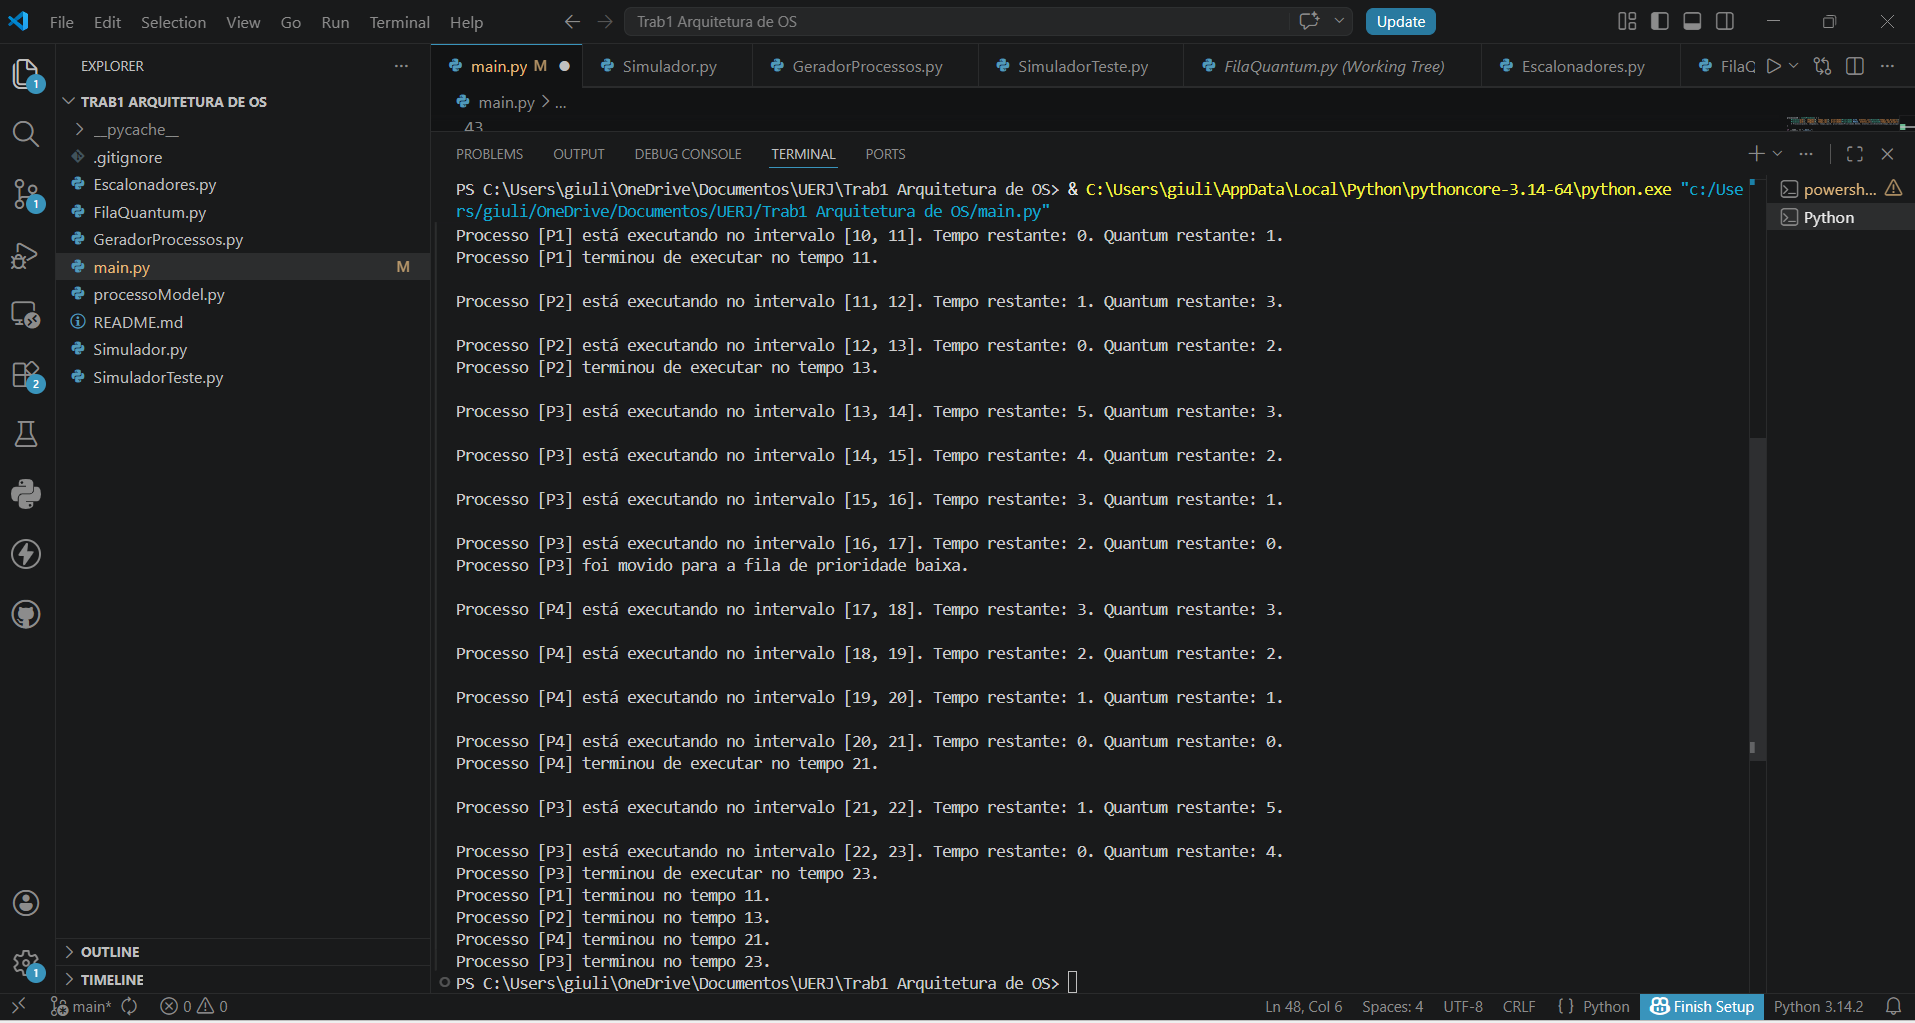
\includegraphics[width=\textwidth]{Passoapassodoprocesso.png}
    \caption{Passo a passo do processo sendo feito.}
    \label{fig:saida_simulador}
\end{figure}

\Figura{saida_sjf.png}
      {Passo a passo da execução com o SJF preemptivo.}
      {fig:saida_sjf}

\Figura{turnaround_final.png}
      {Tabela de turnaround impressa ao final da simulação.}
      {fig:turnaround_final}

\Figura{visualizador.png}
      {Visualizador do simulador, com o gráfico de Gantt e o estado das filas.}
      {fig:visualizador}
%
% Exemplo de figura:
%
% \begin{figure}[H]
%     \centering
%     \includegraphics[width=\textwidth]{saida_simulador.png}
%     \caption{Saída da execução do simulador.}
% \end{figure}
% ============================================================

Ao final da simulação, cada processo possui registrado seu instante de
término.

A partir desse valor é possível calcular seu turnaround utilizando:

\[
T_{turnaround}
=
T_{termino}
-
T_{chegada}
\]

Os logs produzidos durante a execução também permitem acompanhar as
mudanças de estado, a utilização das filas e as operações de entrada
e saída realizadas por cada processo.


% ============================================================
% 13. CONCLUSÃO
% ============================================================

\section{Conclusão}

O desenvolvimento do simulador permitiu aplicar de forma prática os
conceitos relacionados ao gerenciamento e ao escalonamento de
processos em sistemas operacionais.

A estratégia de desenvolver inicialmente uma versão simplificada,
contendo apenas processamento em CPU, mostrou-se útil para validar a
lógica de filas, quantum e preempção antes da introdução de operações
de entrada e saída.

A comparação da implementação inicial do MLFQ com um exemplo
previamente resolvido permitiu verificar a correta evolução do tempo
global e a ordem de execução dos processos.

Após essa validação, a separação entre tempo de CPU e tempo de E/S
permitiu representar processos que alternam entre processamento e
operações bloqueantes, mantendo a CPU disponível para outros processos
durante esses períodos.

A criação de um gerador automático tornou possível produzir cenários
diferentes de execução, variando tempos de chegada, tempos de CPU,
quantidade de eventos de entrada e saída e dispositivos utilizados.

Por fim, os registros produzidos a cada unidade de tempo tornam a
execução do simulador observável e facilitam a compreensão das
decisões realizadas pelo escalonador.


% ============================================================
% REFERÊNCIAS
% ============================================================

\newpage

\begin{thebibliography}{9}

\bibitem{trabalho}
BRUM, Rafaela.
\textit{Trabalho Prático 1 de Arquitetura de Sistemas Operacionais:
Implementando um simulador de escalonamento}.
Universidade do Estado do Rio de Janeiro, 2026.

\bibitem{escalonamento}
BRUM, Rafaela.
\textit{Escalonamento de Processos}.
Material da disciplina Arquitetura de Sistemas Operacionais.
Universidade do Estado do Rio de Janeiro, 2026.

\bibitem{comunicacao}
BRUM, Rafaela.
\textit{Comunicação entre Processos}.
Material da disciplina Arquitetura de Sistemas Operacionais.
Universidade do Estado do Rio de Janeiro, 2026.

\bibitem{exemplo}
BRUM, Rafaela.
\textit{Exemplo de Escalonamento sem E/S}.
Material de exercícios da disciplina Arquitetura de Sistemas
Operacionais.
Universidade do Estado do Rio de Janeiro, 2026.

\end{thebibliography}


\end{document}